\documentclass{beamer}
\usetheme{Singapore}
\usecolortheme{default}

\usepackage[utf8]{inputenc}
\usepackage[T1]{fontenc}
\usepackage{verbatim}
\usepackage{graphics}
\usepackage{listings}
\usepackage{lmodern}

\title{Understanding Git with Alloy}
\subtitle{Milestone 3}
\author{Cláudio Lourenço \and Renato Neves}
\institute{University of Minho\\
Formal Methods in Software Engineering}


\logo{ 
\includegraphics[width=0.15\textwidth]{images/csail_logo.png}
       
\includegraphics[width=0.15\textwidth]{images/uminho_eng_logo.png}}

\begin{document}

\frame {
   \titlepage
}

\frame{
   \frametitle{Table of contents}
   \tableofcontents 
}

\section{Git as VCS}

\begin{frame}
	\frametitle{Git as VCS}
	\begin{block}{Git is one of many Version Control Systems}
		\begin{itemize}
		\item Fast
		\item Efficient
		\item Oriented to snapshots, not differences
		\item Widely used
	\end{itemize}
	\end{block}
\end{frame}
\begin{frame}
   \frametitle{Git as VCS}
   \begin{figure}
      \centering
      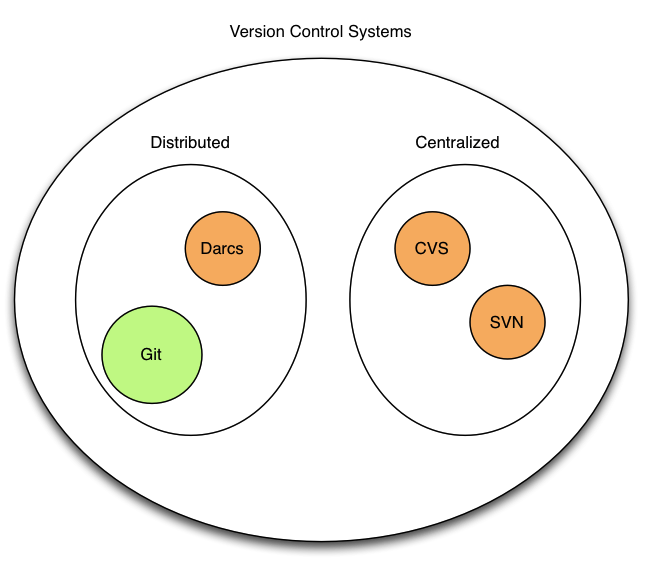
\includegraphics[width=0.5\textwidth]{images/VCS.png}
   \end{figure}
\end{frame}

\section{Project motivation and objectives}
\begin{frame}
	\frametitle{Motivation for this project}
	\begin{block}{Gap in the understanding of Git}
		\begin{itemize}
		\item Lack of precise descriptions
		\item Contradictions in some manuals
		\end{itemize}
	\end{block}
	\begin{block}{An opportunity  appears}
	\begin{itemize}
	\item Developers could benefit from a manual
		that is precise and rigorous
	\end{itemize}
	\end{block}
\end{frame}

\begin{frame}
	\frametitle{The dark world of Git}
	\begin{block}{The common (and above average) knowledge of Git }
	\begin{itemize}
	\item "if there are any uncommitted changes when you run git checkout,
	 Git will behave very strangely." \footnote{"Understanding Git" Manual}
	\item "When you create a branch, it will contain everything
         committed on the branch you created it from at that given
         point. So if you commit more things on the master branch like
         you have done (after creating b), then switch to branch b,
         they won't appear. This is the correct behavior. Does that
         answer your question?" \footnote{An user of Git development 
	 mailing list} 
	\end{itemize}
	\end{block}
\end{frame}

\begin{frame}
	\frametitle{Objectives of this project}
	\begin{block}{Shine some light in Git internals}
		\begin{itemize}
			\item Build a precise model of how Git works, using 
			Alloy
			\item Analyze the model and verify which properties
			does (not) guarantee
			\item Help others to understand Git better, building
			a manual with public access
		\end{itemize}
	\end{block}
\end{frame}


\section{Git internals}

\begin{frame}
   \frametitle{The Git Structure}
   \begin{figure}
      \centering
      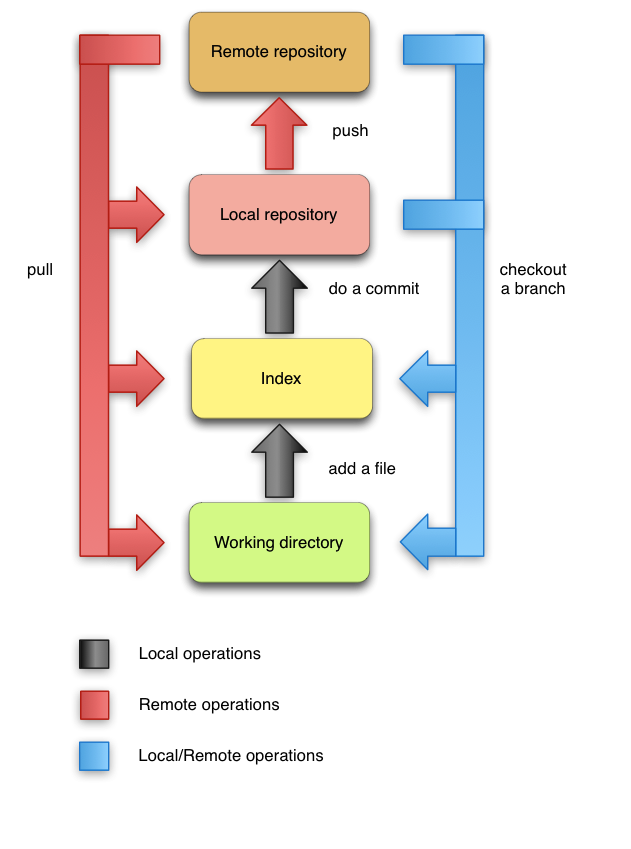
\includegraphics[width=0.45\textwidth]{images/git_workflow.png}
   \end{figure}
\end{frame}

\begin{frame}
   \frametitle{Repository}
   \begin{figure}
      \centering
      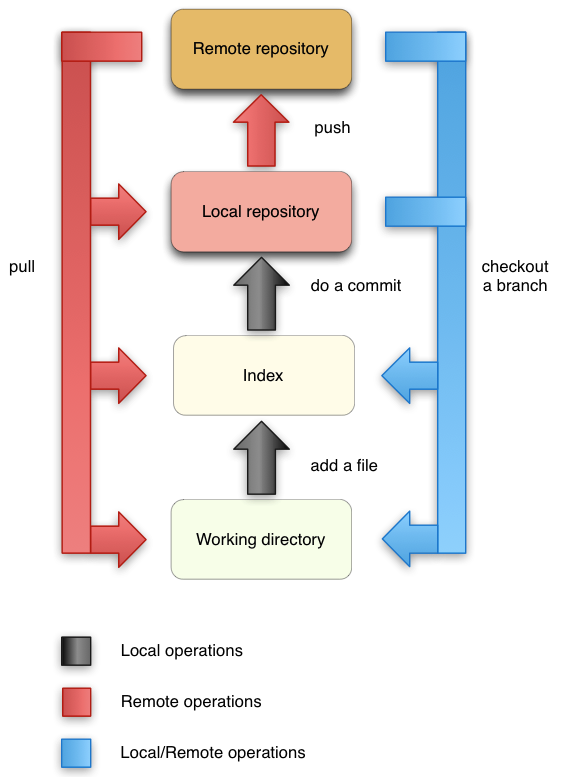
\includegraphics[width=0.4\textwidth]{images/workflow2.png}
   \end{figure}
\end{frame}

\begin{frame}
\frametitle{Repository}
   \begin{figure}
      \centering
      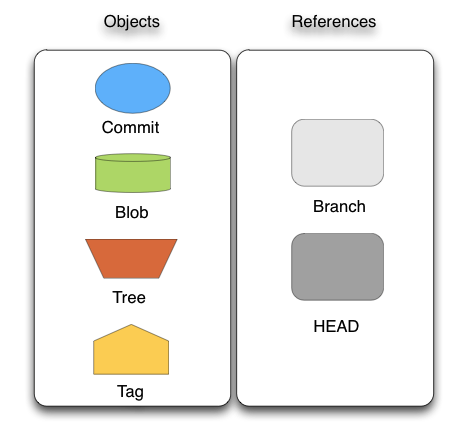
\includegraphics[width=0.5\textwidth]{images/legenda2.png}
   \end{figure}
\end{frame}

\begin{frame}[fragile]
   \frametitle{Blob and Tree}
   \begin{block}{Blob}
      \begin{itemize}
         \item Represents the content of a file
         \item The name is calculated from its content
      \end{itemize}
      \tiny
      \color{blue}
      \begin{lstlisting}
      sig Blob extends Object {}
      \end{lstlisting}
   \end{block}
   \begin{block}{Tree}
      \begin{itemize}
         \item Relation from names to Blobs or/and Trees
         \item Used to represent the file system structure
      \end{itemize}
      \tiny
      \color{blue}
      \begin{lstlisting}
      sig Tree extends Object {
         
         contains: Name -> lone(Tree+Blob)
      
      }
      \end{lstlisting}
   \end{block}
\end{frame}




\begin{frame}[fragile]
   \frametitle{Commit}
   \begin{itemize}
      \item It is like a snapshot of the project on a certain moment
      in time
      \item Author, Committer, Comment - Not important for us
      \item Parent - The Commit which originated the current
      \item Tree - Pointer to a Tree Object
   \end{itemize}
   \tiny
   \color{blue}
   \begin{lstlisting}
                        sig Commit extends Object {
                           points : Tree,
                           parent : set Commit,
                           abs: Path -> Object,
                           merge : set State
                        }
                           
                        sig RootCommit extends Commit {}
\end{lstlisting}
\end{frame}

\begin{frame}[fragile]
\frametitle{Branch and HEAD}
   \begin{block}{Branch}
      \begin{itemize}
         \item It is just a pointer to a commit
      \end{itemize}
   \end{block}
   \begin{block}{HEAD}
      \begin{itemize} 
         \item Special reference that identifies the current Branch
      \end{itemize}
   \end{block}
   \tiny
   \color{blue}
   \begin{lstlisting}
                        sig Branch{
                           marks: Commit lone -> State,
                           branches: set State,
                           head: set State
                        }

                        lone sig Master extends Branch{}
   \end{lstlisting}
\end{frame}

\begin{frame}
	\frametitle{Repository}
	\begin{figure}
		\centering
		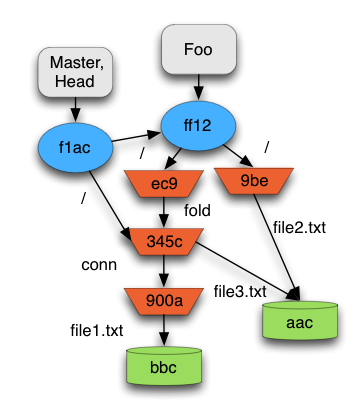
\includegraphics[width=0.4\textwidth]{images/object_assoc.png}
	\end{figure}
\end{frame}

\begin{frame}
   \frametitle{Working Directory}
   \begin{figure}
      \centering
      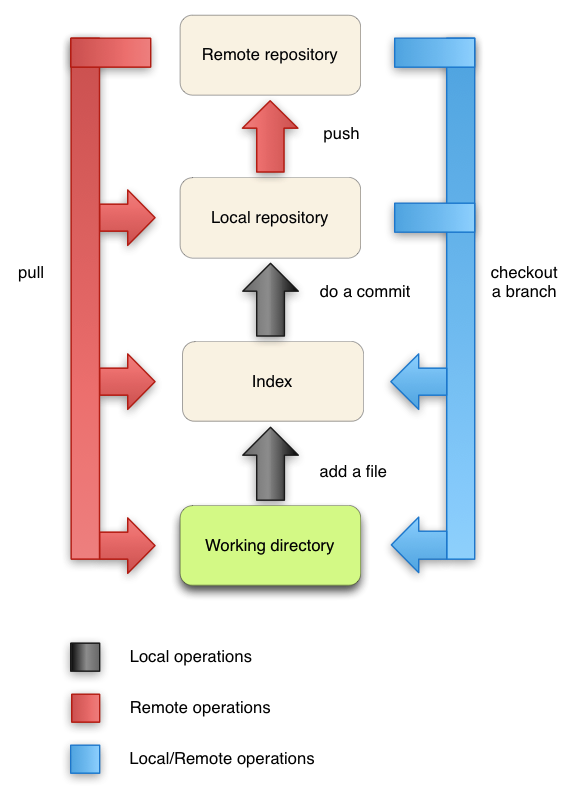
\includegraphics[width=0.4\textwidth]{images/workflow3.png}
   \end{figure}
\end{frame}

\begin{frame}[fragile]
   \frametitle{Working Directory}
   \begin{itemize}
      \item Subset of a file system
      \item Has the content of a project
      \item Files can be the current files or files retrieved
      from the repository
   \end{itemize}
   \tiny
   \color{blue}
   \begin{lstlisting}
                        sig Path {
                           pathparent: lone Path,
                           name: Name,
                           unmerge: set State
                        }

                        one sig Root extends Path{}
   \end{lstlisting}
\end{frame}

\begin{frame}
   \frametitle{Repository}
   \begin{figure}
      \centering
      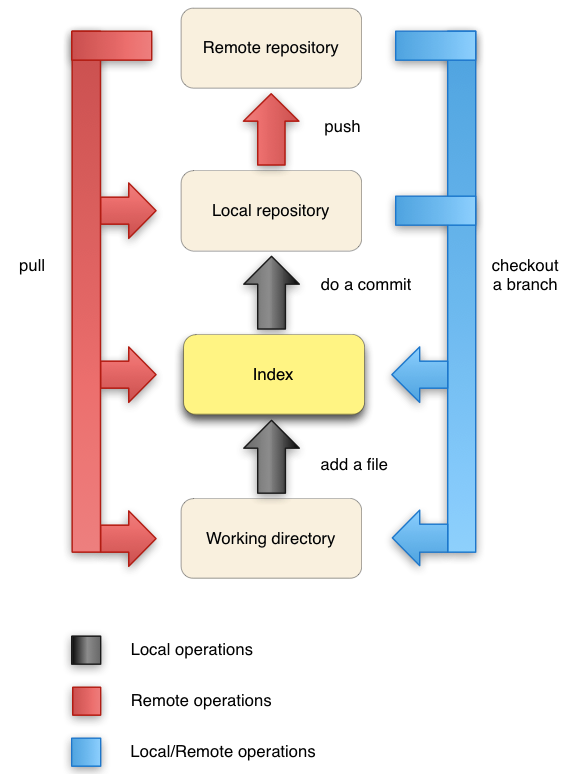
\includegraphics[width=0.4\textwidth]{images/workflow1.png}
   \end{figure}
\end{frame}

\begin{frame}[fragile]
   \frametitle{Index}
   \begin{itemize}
      \item Contains all files that are going to be committed on the next
      commit 
      \item The index is not necessarily equal to the working directory
      \item If an user wants to commit a new file or a newly modified file,
      first he must add it to the index
   \end{itemize}
   \vspace{10mm}
   \tiny
   \color{blue}
   \begin{lstlisting}
                        sig File{
                           path: Path,
                           blob: Blob,
                           index: set State
                        }

   \end{lstlisting}

\end{frame}


\section{Specification of operations}

\begin{frame}[fragile]
   \frametitle{Modeled Operations}
   \begin{itemize}
      \item Add and Remove
      \item Commit
      \item Branch and Branch Remove
      \item Checkout
      \item Merge (2-way and fast-forward)
   \end{itemize}
\end{frame}

\begin{frame}[fragile]
   \frametitle{Add}
   \begin{figure}
      \centering
      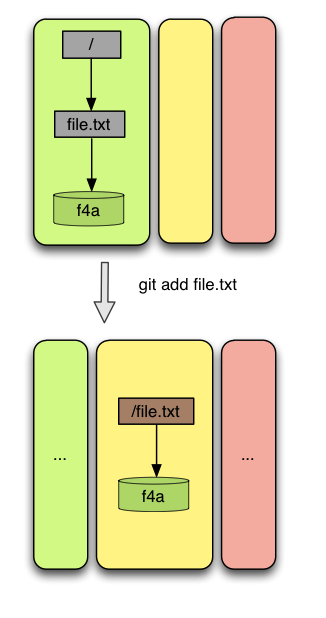
\includegraphics[width=0.3\textwidth]{images/add1.png}
   \end{figure}
\end{frame}

\begin{frame}[fragile]
   \frametitle{Remove}
   \begin{figure}
      \centering
      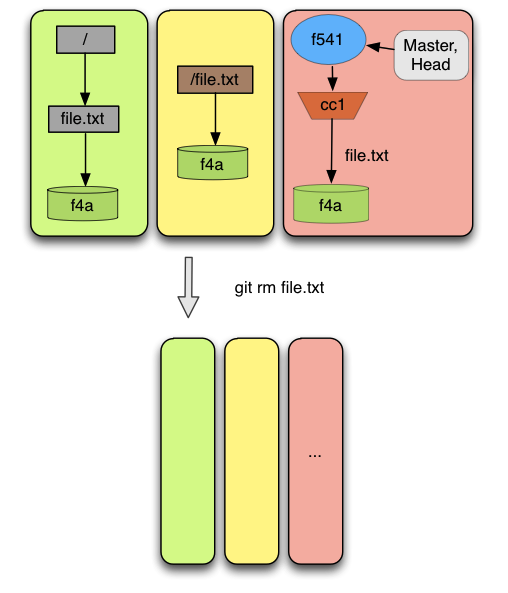
\includegraphics[width=0.45\textwidth]{images/remove1.png}
   \end{figure}
\end{frame}

\begin{frame}[fragile]
   \frametitle{Commit}
   \begin{figure}
      \centering
      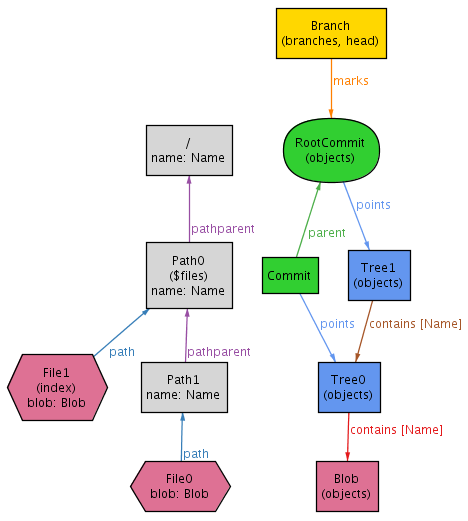
\includegraphics[width=0.45\textwidth]{images/commit1.png}
   \end{figure}
\end{frame}

\begin{frame}[fragile]
   \frametitle{Commit}
   \begin{figure}
      \centering
      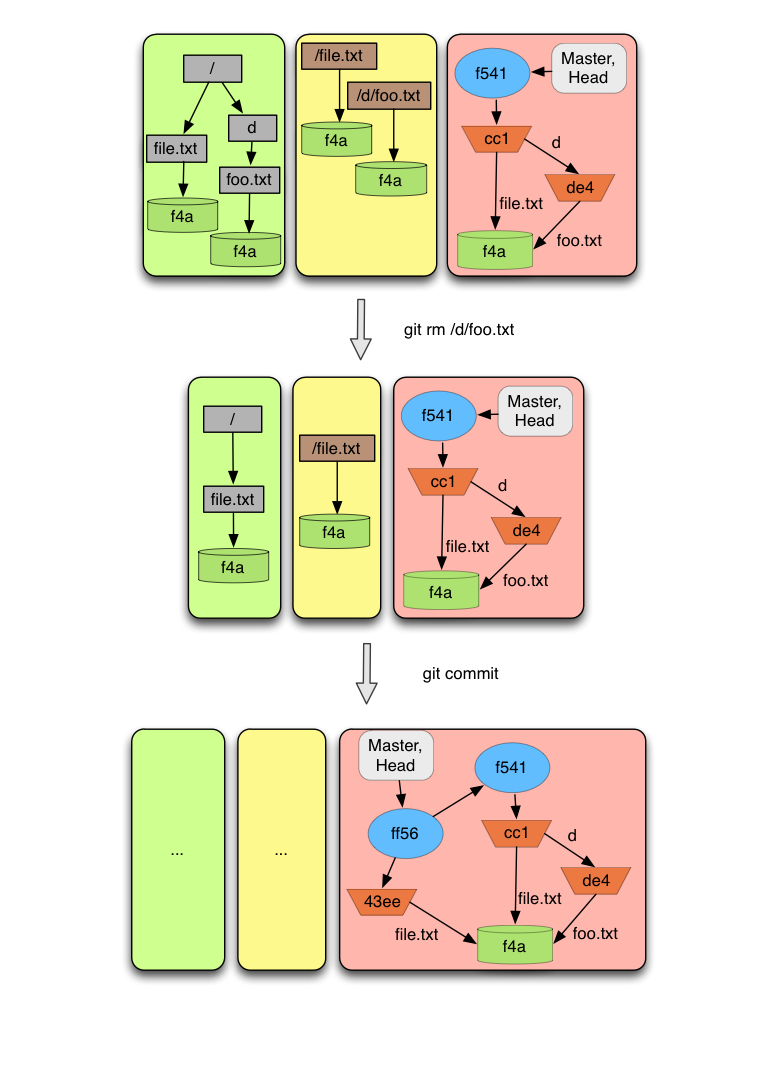
\includegraphics[width=0.45\textwidth]{images/commit2.png}
   \end{figure}
\end{frame}

\begin{frame}[fragile]
   \frametitle{Checkout}
   \begin{figure}
      \centering
      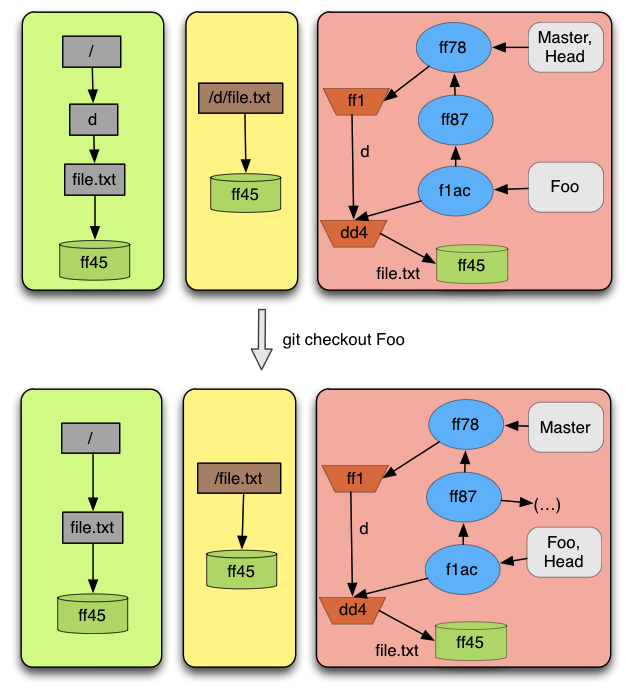
\includegraphics[width=0.45\textwidth]{images/checkout.png}
   \end{figure}
\end{frame}

\begin{frame}[fragile]
	\frametitle{Checkout}
	\begin{block}{The most difficult operation to specify}
	\begin{itemize}
		\item Expected pre-conditions were not found
		\item Instead we found weaker pre-conditions
		\item Strange behaviour caught. Discussed about it 
		with the Git mailing list. Concluded that was a bug
	\end{itemize}
	\end{block}
\end{frame}

\begin{frame}[fragile]
   \frametitle{Pre-conditions found}
\end{frame}

\begin{frame}[fragile]
   \frametitle{ A fast-forward Merge}
   \begin{figure}
      \centering
      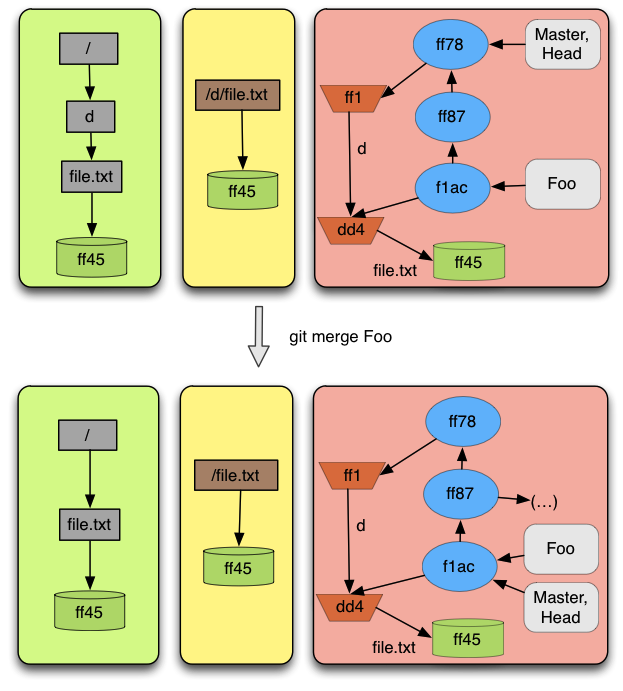
\includegraphics[width=0.45\textwidth]{images/fastforwardmerge.png}
   \end{figure}
\end{frame}

\begin{frame}[fragile]
   \frametitle{A 2-way Merge}
   \begin{figure}
      \centering
      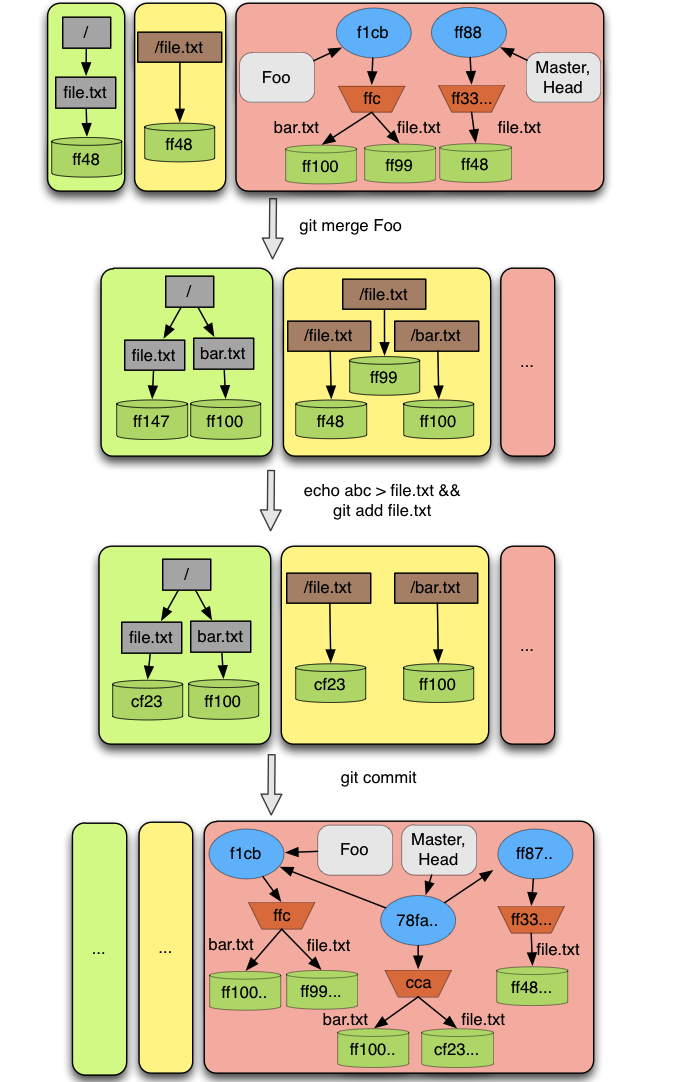
\includegraphics[width=0.45\textwidth]{images/merge2way.png}
   \end{figure}
\end{frame}

\begin{frame}[fragile]
   \frametitle{A 3-way Merge}
   \begin{figure}
      \centering
      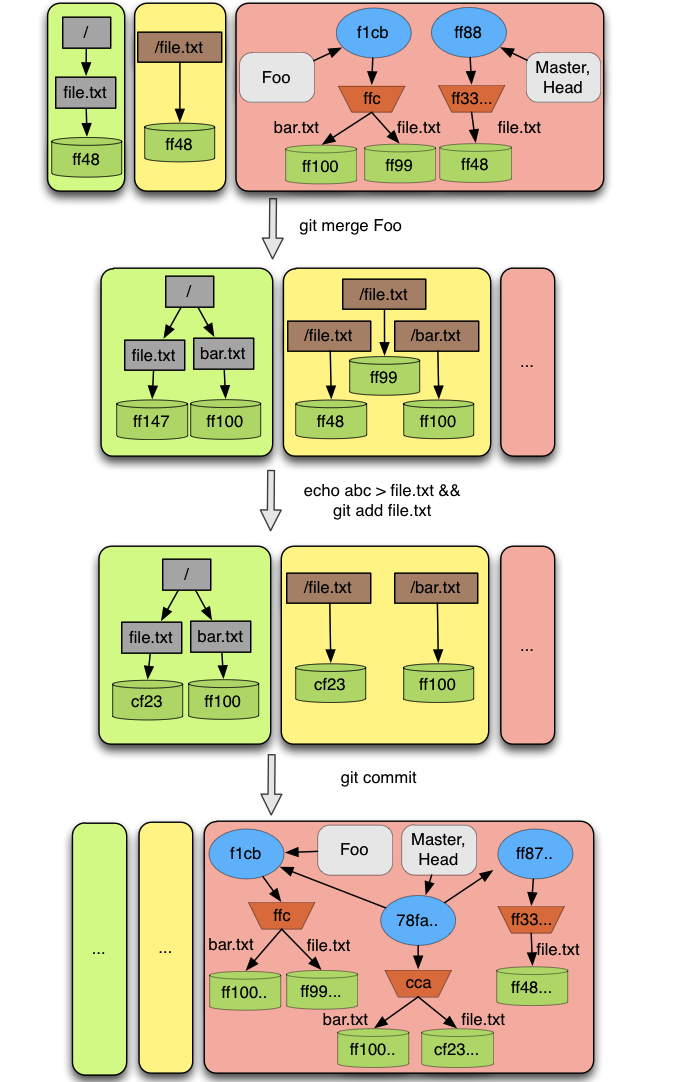
\includegraphics[width=0.45\textwidth]{images/merge2way.png}
   \end{figure}
\end{frame}

\begin{frame}[fragile]
	\frametitle{Merge}
	\begin{block}{The la la} 
	\begin{itemize}
		\item aaawith the Git mailing list. Concluded that was a bug
	\end{itemize}
	\end{block}
\end{frame}

\begin{frame}[fragile]
	\frametitle{Merge}
	\begin{block}{The la la} 
	\begin{itemize}
		\item aaawith the Git mailing list. Concluded that was a bug
	\end{itemize}
	\end{block}
\end{frame}

\section{Documentation}

\begin{frame}
	\frametitle{Website}
	\begin{itemize}
	\item Website created based on the manual 
	\item http://nevrenato.github.com/CSAIL\_Git
	\end{itemize}

\end{frame}

\section{Conclusion}

\begin{frame}
	\frametitle{Future Work}
	\begin{itemize}
	\item Model more operations (rebase, fetch, 3-way merge...) 
	\item Specify more properties that the model does (not) guarantee
	\item Build interactive diagrams of concrete examples of operations 
	\end{itemize}
\end{frame}

\begin{frame}
	\frametitle{Conclusions}
\end{frame}


\end{document}
